\chapter{Unit Tests}
Die Unit Tests von Morik wurden so geschrieben, dass sie uns beim Entwickeln neuer Funktionalitäten helfen. Als Test-Framework wird dabei \href{https://github.com/moorts/Morik/blob/main/src/CMakeLists.txt#L24}{\textit{GoogleTest}} verwendet. Um eine gute Übersicht über die Tests zu haben, sind diese genau in der gleichen Ordnerstruktur angeordnet wie der Produktivcode, nur eben im \href{https://github.com/moorts/Morik/tree/main/src/tests}{\textit{tests}}-Ordner. Im Folgenden wird genauer auf die Umsetzung der ATRIP-Regeln, das Messen der Code Coverage und den Einsatz von Mock-Objekten eingegangen.

\section{ATRIP-Regeln}
Diese Regeln definieren eine Reihe von Eigenschaften, die gute Unit Tests erfüllen sollten. ''ATRIP'' steht dabei für automatic, thorough, repeatable, independent und professional. Automatic, repeatable und independent sind dabei harte Regeln, was bedeutet, dass diese Eigenschaften messbar sind, während thorough und professional weiche Regeln sind, sodass diese nur bedingt messbar sind. Im Folgenden wird näher auf die einzelnen Regeln und deren Erfüllung seitens Morik eingegangen.

\subsection{Automatic}
Die Tests laufen alle eigenständig ab. Es gibt also keinen Test, der bspw. eine Eingabe erwartet. Außerdem prüfen die Tests ihre Ergebnisse selbst, indem Assertions verwendet werden. Dadurch gibt es eine deutliche Übersicht, ob alle Tests erfolgreich ausgeführt wurden, statt dass die Auswertung, ob der Test das richtige Ergebnisse produziert hat, manuell durchgeführt werden muss.

\subsection{Thorough}
Diese Regel besagt, dass alles Notwendige des Systems getestet ist. Dies erfüllt Morik nicht, da hierfür mehr Tests benötigt werden. Wir haben uns beim Schreiben der Tests jedoch trotzdem auf das Testen der wichtigen Funktionalitäten fokussiert. Demnach testen die bestehenden Tests hauptsächlich das Ver- und Entschlüsseln der Passwörter (bspw. bei den \href{https://github.com/moorts/Morik/blob/main/src/tests/application/encryptor_tests.cpp}{\textit{encryptor\_tests}}), sowie das Lesen dieser aus der Datenbank (bspw. bei den \href{https://github.com/moorts/Morik/blob/main/src/tests/application/repository_tests.cpp}{\textit{repository\_tests}}). Dies sind die wesentlichen Bestandteile eines Passwort Managers, jedoch werden auch hiervon nicht alle Aspekte getestet. Auf eine Einschätzung wie ''gründlich'' die Tests tatsächlich sind, wird in der Sektion ''Code Coverage'' eingegangen.

\subsection{Repeatable}
Unsere Tests sind wiederholbar. Sie können also immer wieder ausgeführt werden und liefern immer das gleiche Ergebnis, sofern keine Änderungen am Code vorgenommen wurden. Dies liegt daran, dass die Tests nicht von äußeren Umständen abhängen. Weitere Einblicke wie wir die Tests von äußeren Abhängigkeiten lösen, werden in der Sektion ''Mocks'' gegeben.

\subsection{Independent}
Jeder unserer Tests testet eine dedizierte Funktionalität wie bspw. das Lesen eines Eintrags aus der Datenbank oder das Ver- und Entschlüsseln von Passwörtern. Hierbei wird das Ver- und Entschlüsseln, wie man in \href{https://github.com/moorts/Morik/blob/main/src/tests/plugins/encryption/crypto_tests.cpp}{\textit{crypto\_tests}} sieht, als eine Funktionalität aufgefasst, da man ein Passwort nur entschlüsseln kann wenn es zuvor verschlüsselt wurde und das Verschlüsseln eines Passworts ohne die Intention es wieder zu entschlüsseln sinnfrei ist. Da jeder Test genau eine Funktionalität testet, gibt es keine Abhängigkeiten zwischen den Tests, weshalb auch die Ausführungsreihenfolge irrelevant ist.

\subsection{Professional}
Der Testcode von Morik ist professionell geschrieben. Dies bedeutet, dass er leicht verständlich ist aufgrund von sprechenden Bezeichnern und dem Befolgen der AAA-Normalform. Außerdem werden keine unrelevanten Aspekte der Applikation getestet, sondern wir fokussieren uns, wie bereits bei ''Thorough'' genannt, auf das Testen der wichtigsten Funktionalitäten.

\section{Code Coverage}
\begin{figure}[ht]
	\centering
	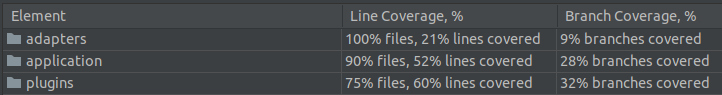
\includegraphics[width=1.0\textwidth]{Bilder/coverage.png}
	\caption{Line Coverage und Branch Coverage Messung}
	\label{fig:coverage}
\end{figure}

Wie zuvor bereits genannt, ermöglicht die Code Coverage eine Einschätzung wie ''gründlich'' die Tests tatsächlich sind, indem gemessen wird wie viel Code beim Testen durchlaufen wird im Vergleich zu wie viel Code insgesamt in der kompletten Applikation durchlaufen werden kann. Hierbei werden zwei Metriken besonders häufig verwendet. Zum einen gibt es die Line Coverage, die die ausgeführten Codezeilen zählt, während es zum anderen die Branch Coverage gibt. Diese zählt die ausgeführten Verzweigungsmöglichkeiten. Dabei ist letztere Metrik aussagekräftiger für die tatsächliche ''Gründlichkeit'' der Tests, während die Line Coverage allerdings leichter zu messen ist. Dass die Branch Coverage aussagekräftiger ist, kommt vor Allem daher wie einfach es ist die Line Coverage zu erhöhen. Beispielsweise könnte eine Funktion, welche tatsächlich getestet wird, so umgeschrieben werden, dass sie mehr Zeilen Code einnimmt. Dadurch steigt die Line Coverage, da der getestete Code relativ gesehen nun einen größeren Anteil der gesamten Codebasis einnimmt als zuvor. Die Branch Coverage jedoch steigt nicht, da sich nichts daran geändert hat welche Funktionen aufgerufen werden oder welche Verzweigungen innerhalb der Funktion tatsächlich durchlaufen werden.\\
Wie in \autoref{fig:coverage} gezeigt, erreicht Morik mit den Tests eine Line Coverage von 44.3\%, während eine Branch Coverage von nur 23\% erreicht wird. Dies zeigt erneut, dass es einfacher ist eine hohe Line Coverage zu erreichen, als eine hohe Branch Coverage. \todo{Zahlen und screenshot anpassen} Ermittelt werden diese Zahlen durch das Ausführen der Tests mit Coverage mithilfe von JetBrains IDE CLion.

\section{Mocks}
Einige der Klassen von Morik sind abhängig von anderen Klassen, um richtig funktionieren zu können. Um diese Klassen jedoch trotzdem testen zu können, ohne vorher alle Abhängigkeiten konstruieren zu müssen, werden an ausgewählten Stellen Mock-Objekte eingesetzt. Für das Erzeugen der Mock-Objekte wird \textit{gmock} verwendet, das in GoogleTest enthalten ist. So kann in der Klasse \href{https://github.com/moorts/Morik/blob/main/src/tests/application/AbstractDatabaseInterfaceMock.h}{\textit{AbstractDatabaseInterfaceMock}} bspw. das Mocken eines AbstractDatabaseInterface beobachtet werden, sodass in \href{https://github.com/moorts/Morik/blob/main/src/tests/application/repository_tests.cpp}{\textit{repository\_tests}} die EntryRepository getestet werden kann, die die Übergabe eines AbstractDatabaseInterface im Konstruktor erwartet. Ein weiteres Mock-Objekt ist das \href{https://github.com/moorts/Morik/blob/main/src/tests/adapters/database/AbstractSqlDatabaseMock.h}{\textit{AbstractSqlDatabaseMock}}, das eine AbstractSqlDatabase mockt. Dies wird verwendet, um in \href{https://github.com/moorts/Morik/blob/main/src/tests/adapters/database/databaseInterface_tests.cpp}{\textit{databaseInterface\_tests}} den DatabaseInterface-Adapter testen zu können, der wiederum die Übergabe einer AbstractSqlDatabase im Konstruktor erwartet.
